\section{Естественный язык как модальность данных и примененимость методов машинного обучения}
\subsection{Специфика репрезентации данных}
Как уже было сказано, обработка естественного языка NLP одна из самых актуальных в настоящее время. Выше было отмечено, что NLP это сложный процесс, ключевыми сложностями вызванными непосредственно природой данных, являются кодирование данных и работа с непостоянной размерностью. Фраза на естественном языке - это последовательность слов некоторого языка, но для любого алоритма потребуется каким-то образом перевести ее в числовой тип, единственный принимаеиый существующими алгоритмами. Слова крайне враждебны в этом отношении, наивные методы крайне неэффективны, и, чтобы покрыть целый словарь, понадобится очень много памяти, более того, фраза даже из закодированных слов имеет нефиксированную длину. 
В итоге при подготовке данных для решения встает два вопроса:
\begin{itemize}
    \item Какой метод кодирования слов оптимален в терминах сохранения информации и эффективности хранения
    \item Как обработать последовательность нефиксированной длины или преобразовать ее таким образом, чтобы размерность данных стала фиксированной
\end{itemize}
Последний вопрос еще более важен, так как он непосредственно связан с моделью для решения задачи.
\subsection{Механизмы кодирования и репрезентации в качестве многомерных объектов}
Для какой-либо задачи в области NLP будет определен некоторый конечный словарь - множество всех допустимых встречающихся слов естественного языка. Очевидным методом является применение кодирования OneHotEncoding (далее OHE), при котором $i$-ому слову будет соответсвовать вектор состоящий из нулей с $i$-ым элементом единицей, то есть: 
\begin{equation} \label{ohe_eq} 
\text{\textit{Для словаря}}\ V, |V| = N \ \exists \ ohe:V \longrightarrow \mathds{R}^{N}; ohe(V_{i}) = a, \forall j \neq i a_{j}=0,\ a_{i} = 1 
\end{equation}

Отображение \ref{ohe_eq} позволяет получить численное представление слов в виде векторов, однако размерность равна таковой у словаря.

От части эту проблему можно решить при помощи грамотного разделения фраз на слова. Вместо наивного разбиения на непосредственные слова (разделенные в языке пробелами) и знаки пунктуации можно сократить длину словаря при помощи \textit{токенизации}. Алгоритмы токенизации могут быть разными, помимо сокращения мощности множества слов токенизация может так же сообщать полезную информацию алгоритмы, как будет показанно позже. \newline
Как самостятельный контейнер информации one-hot вектор не несет смысла, кроме явного указания на то, что за слово было закодировано. Полезным преобразованием является векторизация слова (Word To Vector - далее W2V)\cite{w2v}. W2V является обучаемой системой, которая отображает токены в вектора фиксированной размерности, являющейся гиперпараметром. В итоге обучения получается матрица весов $W_{N \times S}$, алгоритм устроен таким образом, что при помощи прохода окном по послеовательности токенов, максимизируются условные вероятности появления слова из центра окна в окржении остальных слов из окна. Таким образом, выявляется контекстная значимость слов. Векторы полученные данным алгоритмом обладают удобными свойствами, в частности компактность относительно семантического значения, то есть блзкие по смысловому значению слова отобразятся в близкие векторы. 
\begin{equation} \label{w2v} 
\text{\textit{Для словаря}}\ V, |V| = N \ w2v_{S}:V \longrightarrow \mathds{R}^{S},\ S \in \mathds{N};
w2v_{S}(V_{i}) = ohe(v_{i})\times W_{N \times S} = b \in \mathds{R}^{S}
\end{equation}
Усовершенствованием технологии является FastText \cite{ft} помимо улучшенного процесса обучения применяющий дополнительно подобие токенизации, разбивая слова на части. Это позволяет более эффективно обрабатывать неизвестные слова, так как они могут состоять из встреченных ранее токенов, и выделяет больше информации за счет работы с уровнем, ниже слов естесвенного языка.
Таким образом, для работы классических методов машинного обучения можно получить векторное представление фразы в виде последовательности векторов, а затем каким либо образом преобразовать в единственный вектор при помощи поэлементного среднего:
\begin{align*} 
x = \frac{ \sum_{i=1}^{M} v2w_{S}(v_{i}) }{M} \in \mathds{R}^{S}
\end{align*}
Для методов глубинного обучения инструментарий кодирования может использоваться такой же, однако для наиболее эффективных и рассмотренных далее в работе архитектур он немного отличается. Важно отметить, что методы глубинного обучения обыкновенно оперируют всей последовательностью, не сводя ее к одному вектору. Как было отмечено в \cite{RNN_survey}, возможность оперировать всей последовательностью позволяет захватывать конекст последовательности, несмотря на очевидные плюсы алгоритмов, инвариантных к длине данных, они проигрывают в сфере восприятия и выделения черт (feature extraction).

Применяются достаточно продвинутые алгоритмы токенизации. BPE-токенизация \cite{bpe} применяется во многих популярных и мощных решениях, алгоритм очень эффективен засчет отыскания и жадного перекодирования наиболее частых пар токенов в новый токен, не встречавшийся ранее. Как и BPE Word Piece токенизация, впервые представленныя в \cite{word_piece}, разбивает последовательность на уровне ниже целых слов. Метод является усовершенствованной версией и вместо частоты в BPE оперирует вероятностным подходом. При выборе пар высчитывается правдоподобие - вероятность последовательного нахождения токенов друг за другом. Word Piece добавляет токены в словарь склеивая входные до тех пор, пока уровень правдоподобия не опустится до заранее выбранного порогого значения. Алгоритм так же является жадным, но в отличие от BPE итерации заданы не напрямую, а через выше обозначенный порог. 

Для векторизации токенов в нейронных сетях используют так же слой вложения (Embedding). Итоговое вычисление вложенного представления схоже с \ref{w2v}. Блок препроцессинга включен в саму сеть и обучается вместе с ним, от обычного линейного он также отличается оптимизацией для работы с разреженными данными.
При кодировании последовательности может оказаться так, что одинаковые векторы стоят на разных местах, то есть один и тот же токен может выполнять разную роль в одной фразе. Чтобы добавить информацию об относительном положении слова в последовательности, к каждому вектору добавляется значение полученное из позиционного кодирования (Positional Encoding или PE) поэлементным сложением. Значения вычисляются следующим образом \cite{transformer}\cite{pe}:\\
\textit{Пусть t - позиция в последовательности, d - размерность векторного представления, (i) - индекс элемента вектора} 
\begin{align*}
p_{t}^{(i)} = f(t)^{(i)} := 
\begin{cases} 
sin(w_{k} * t), & \textit{при } i=2k 
\\
cos(w_{k} * t), & \textit{при } i=2k +1
\end{cases}
\textit{, где }
w_{k} = \frac{1}{1000^{2k/d}}
\end{align*}
\newline
Пример полученных значений - \ref{pe_vals}.
\begin{figure}[h]
\caption{Спектр значений позиционного кодирования с размерностью (Depth) 128 и максимальной длинной (Position) 50, каждая строка - вектор $p_{t}$}
\centering
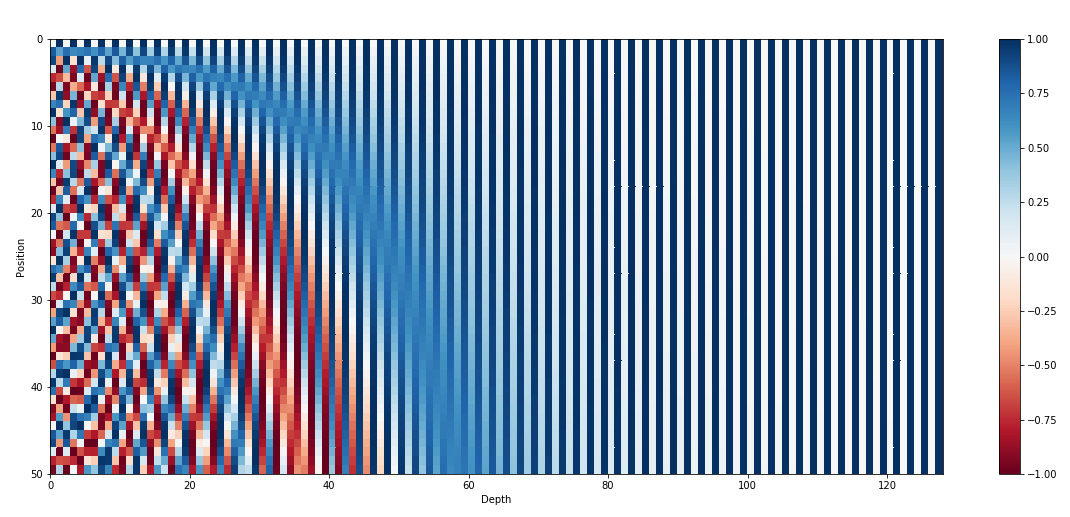
\includegraphics[width=1\textwidth]{positional_encoding.png}
\label{pe_vals}
\end{figure}
\newline